\section{Statistical Analysis}

% The filename of each non-segmented brain MRI contains the age of the subject. Compute the correlation between brain volume and age as well as between white matter, grey matter ratio and age, and state the model assumptions [5]. For each correlation, compute its statistical significance [5].

% Repeat the same experiments by normalising the brain volume by the total intracranial volume (white matter, grey matter and cerebrospinal fluid) [5]. What conclusions can you drawn from these analyses [10]?

The volume of each segmented tissue for the unsegmented subjects can be calculated using the corresponding NIfTI headers, which contains information about voxel dimensions. Once the volumes have been calculated, they can be compared to the subjects ages, as shown in Figure \ref{fig:volumes-correlations}, where normalised volumes mean tissue volume divided by intracranial volume (ICV), which is the addition of CSF, GM and WM volumes. No correlation has been found between the ages and WM/GM ratio ($R = 0.09$, $p = 0.706$).

The most significant correlation ($R = -0.52$, $p = 0.018$) is the one for age vs. normalised brain volume (i.e. (GM + WM) / ICV). A negative Pearson correlation ratio indicates that the size of the brain in relation to the skull decreases with age. This seems to be due to the fact that WM is also reduced with age ($R = -0.44$, $p = 0.055$), although this relation is less significant. Results in first row of Figure \ref{fig:volumes-correlations} indicate that absolute brain volume is independent of age. To calculate the Pearson's correlations, it has been assumed that ages and volumes are normally distributed.

\begin{figure}
  \centering
  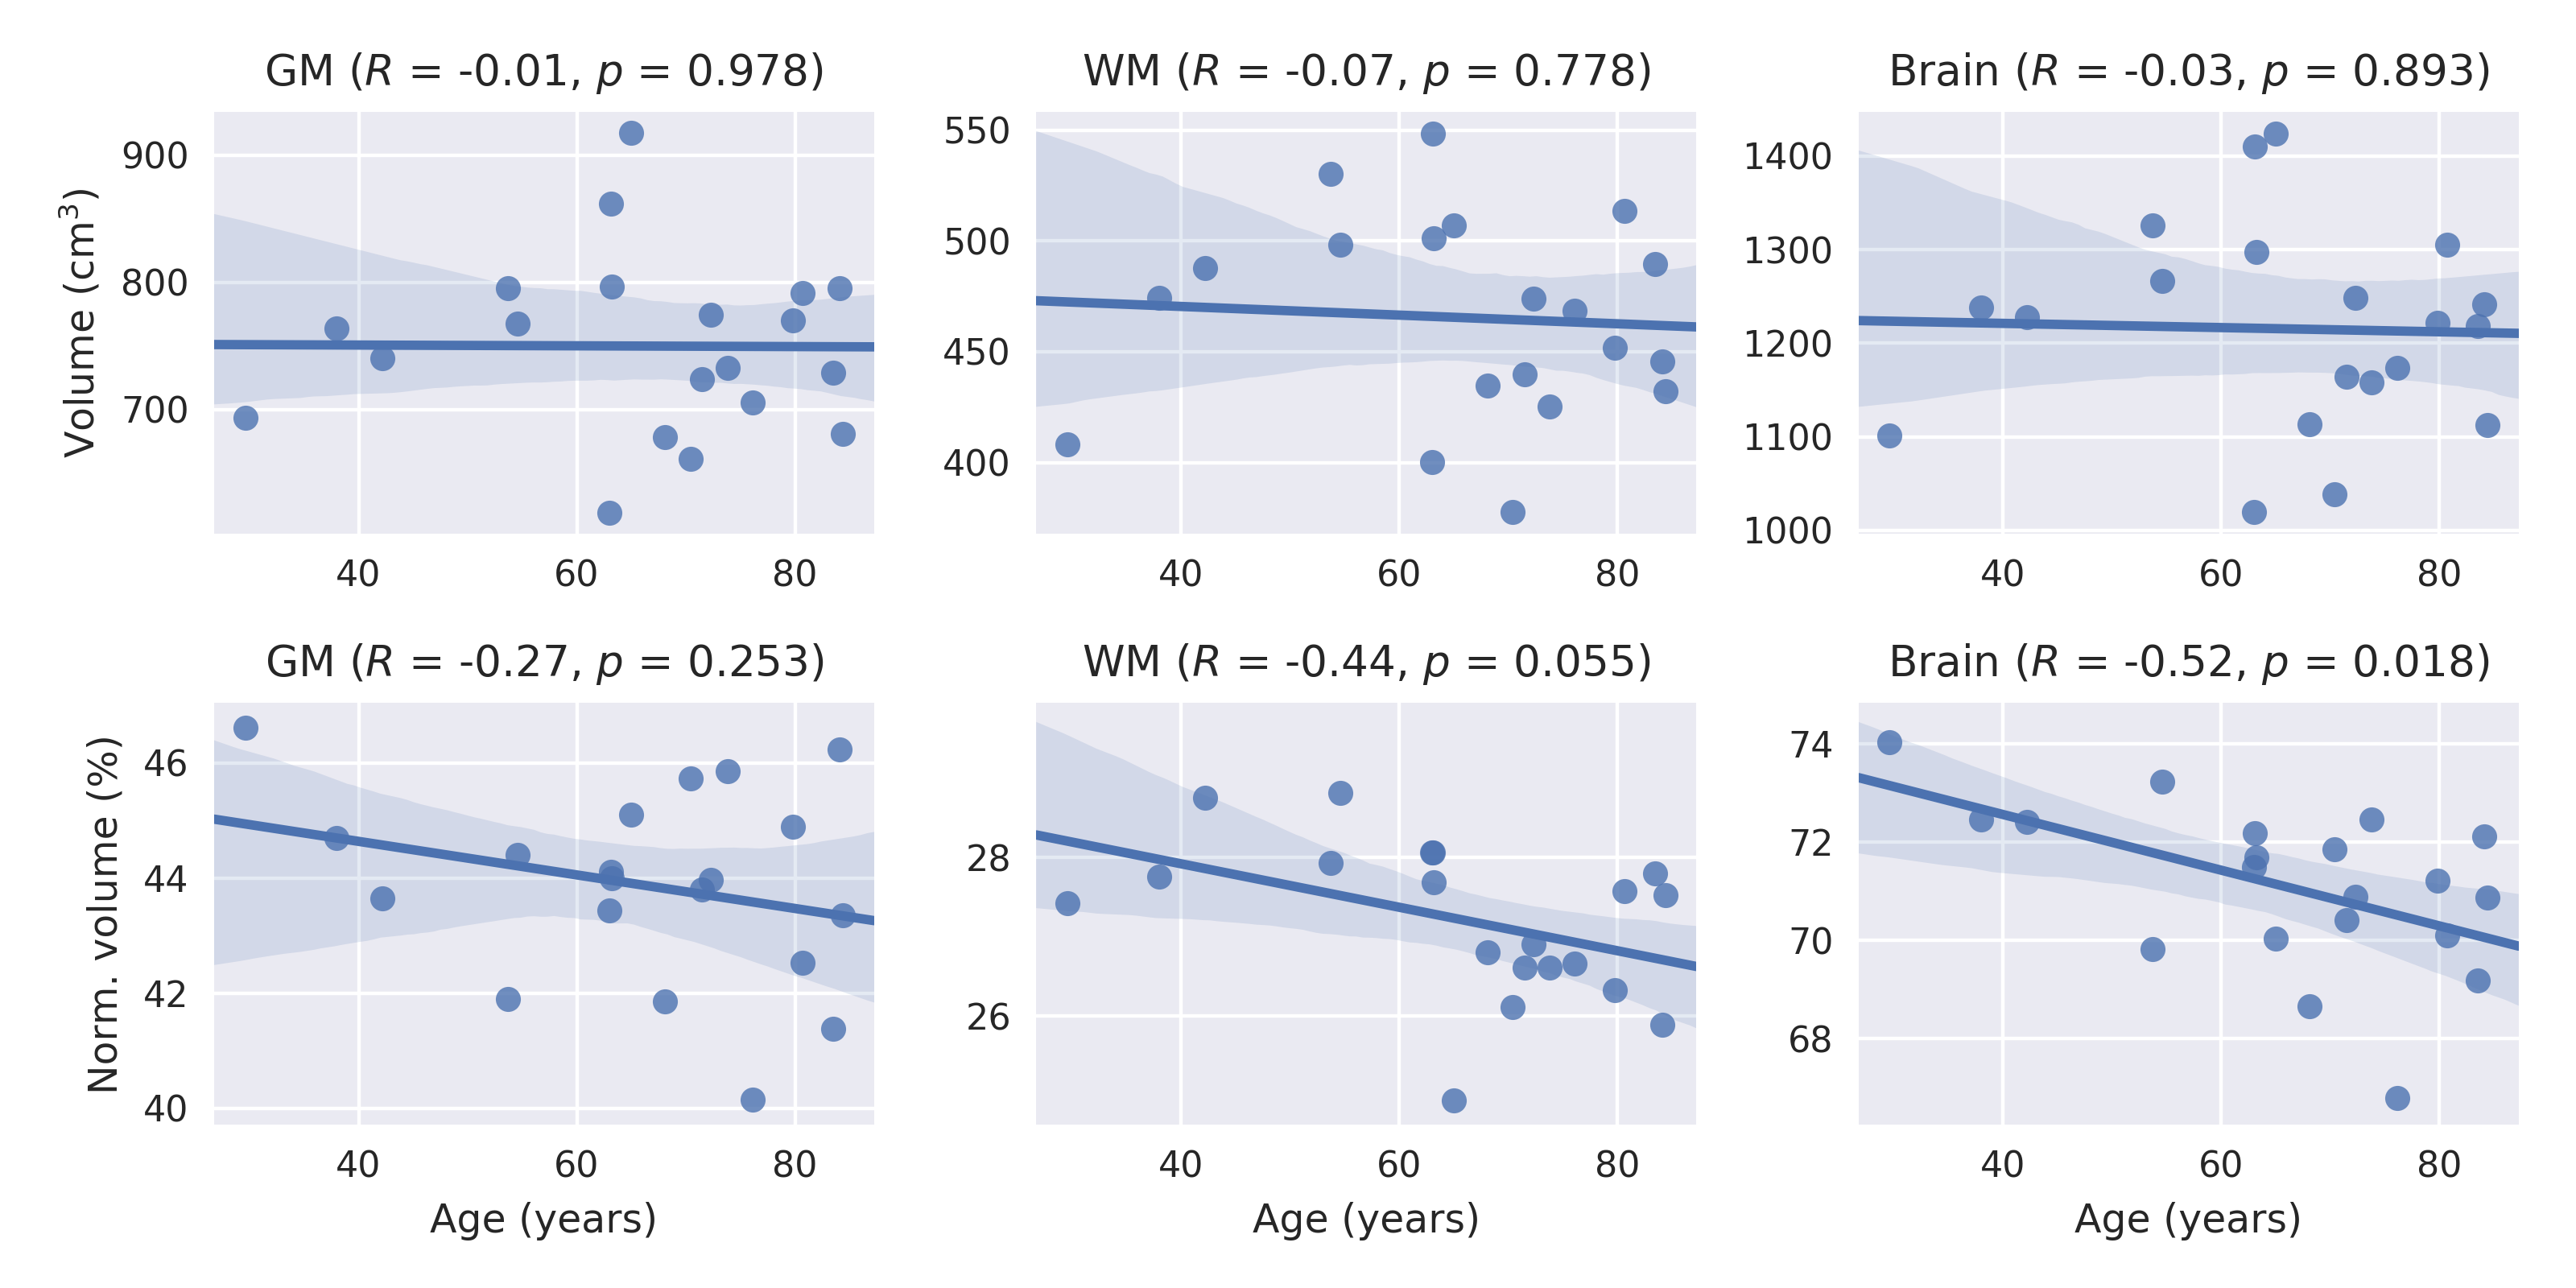
\includegraphics[width=\textwidth]{figures/volumes_stats}
  \caption{Correlations between age and segmented tissue volumes. Top row: volumes in cm$^3$; bottom row: normalised volumes (i.e. divided by ICV). Brain volume is calculated as GM volume + WM volume. $R$ is the Pearson correlation coefficient and $p$ is the two-tail p-value for testing non-correlation. Dots represent individual subjects; lines represent regression models; shaded areas represent 95\% confidence intervals.}
  \label{fig:volumes-correlations}
\end{figure}
